\documentclass[tikz, border=10pt]{standalone}
\usepackage{pgfplots}
\pgfplotsset{compat=1.18}
\usepackage{sfmath}
\begin{document}
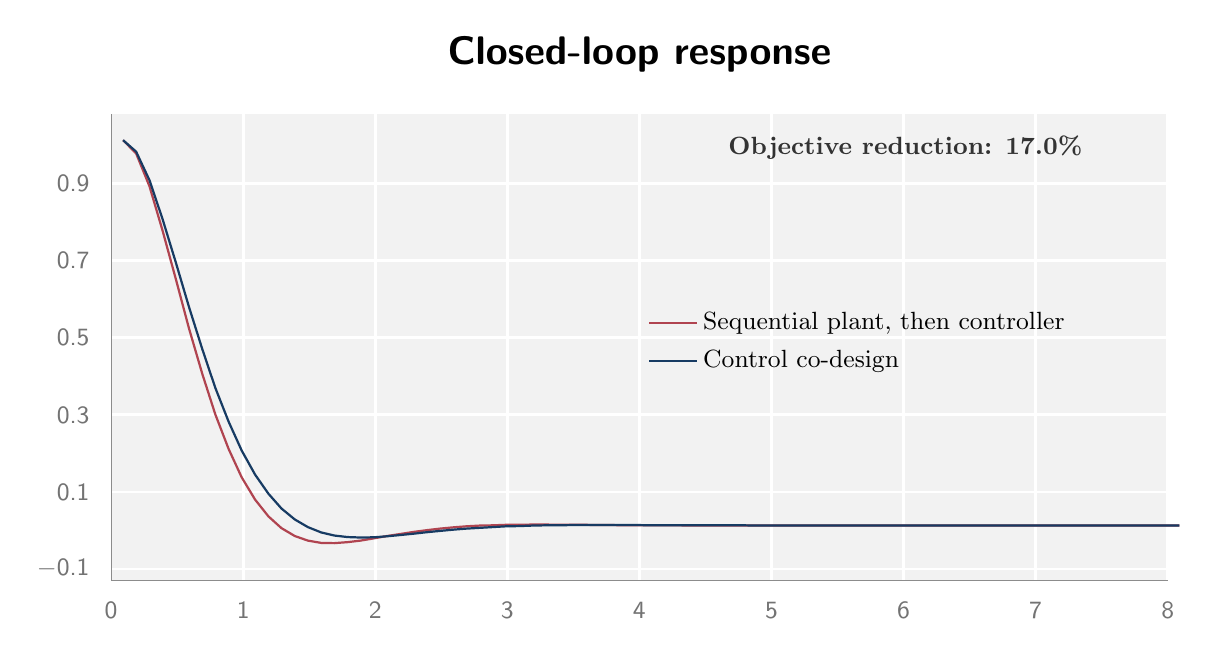
\begin{tikzpicture}[font=\sffamily]

\def\SEQcoords{(0.0907,1.0132) (0.1895,0.9788) (0.2906,0.8934) (0.3893,0.7788) (0.4904,0.6523) (0.5892,0.5251) (0.6903,0.4066) (0.789,0.3013) (0.8901,0.2112) (0.9889,0.1377) (1.09,0.0801) (1.1911,0.0364) (1.2898,0.0059) (1.3909,-0.0146) (1.4897,-0.0265) (1.5908,-0.0325) (1.6895,-0.0331) (1.7906,-0.0305) (1.8894,-0.0265) (1.9905,-0.0206) (2.0892,-0.0146) (2.1903,-0.0093) (2.2891,-0.004) (2.3902,0.0006) (2.4889,0.0046) (2.59,0.0079) (2.6888,0.0106) (2.7899,0.0125) (2.891,0.0132) (2.9897,0.0145) (3.0908,0.0145) (3.1896,0.0152) (3.2907,0.0152) (3.3894,0.0145) (3.4905,0.0145) (3.5893,0.0145) (3.6904,0.0139) (3.7891,0.0139) (3.8902,0.0132) (3.989,0.0132) (4.0901,0.0132) (4.1888,0.0132) (4.2899,0.0132) (4.391,0.0125) (4.4898,0.0125) (4.5909,0.0125) (4.6896,0.0125) (4.7907,0.0125) (4.8895,0.0125) (4.9906,0.0125) (5.0893,0.0125) (5.1904,0.0125) (5.2892,0.0125) (5.3903,0.0125) (5.489,0.0125) (5.5901,0.0125) (5.6889,0.0125) (5.79,0.0125) (5.8911,0.0125) (5.9898,0.0125) (6.0909,0.0125) (6.1897,0.0125) (6.2908,0.0125) (6.3895,0.0125) (6.4906,0.0125) (6.5894,0.0125) (6.6905,0.0125) (6.7892,0.0125) (6.8903,0.0125) (6.9891,0.0125) (7.0902,0.0125) (7.1889,0.0125) (7.29,0.0125) (7.3888,0.0125) (7.4899,0.0125) (7.591,0.0125) (7.6897,0.0125) (7.7908,0.0125) (7.8896,0.0125) (7.9907,0.0125) (8.0891,0.0125)}

\def\CCDcoords{(0.0907,1.0132) (0.1895,0.9834) (0.2906,0.9093) (0.3893,0.8086) (0.4904,0.6953) (0.5892,0.5808) (0.6903,0.4708) (0.789,0.3702) (0.8901,0.2821) (0.9889,0.2073) (1.09,0.145) (1.1911,0.0953) (1.2898,0.0569) (1.3909,0.0284) (1.4897,0.0086) (1.5908,-0.0053) (1.6895,-0.0133) (1.7906,-0.0173) (1.8894,-0.0185) (1.9905,-0.0179) (2.0892,-0.0153) (2.1903,-0.012) (2.2891,-0.0086) (2.3902,-0.0047) (2.4889,-0.0014) (2.59,0.0019) (2.6888,0.0046) (2.7899,0.0066) (2.891,0.0086) (2.9897,0.0106) (3.0908,0.0112) (3.1896,0.0125) (3.2907,0.0132) (3.3894,0.0132) (3.4905,0.0139) (3.5893,0.0139) (3.6904,0.0139) (3.7891,0.0139) (3.8902,0.0139) (3.989,0.0139) (4.0901,0.0132) (4.1888,0.0132) (4.2899,0.0132) (4.391,0.0132) (4.4898,0.0132) (4.5909,0.0132) (4.6896,0.0132) (4.7907,0.0132) (4.8895,0.0125) (4.9906,0.0125) (5.0893,0.0125) (5.1904,0.0125) (5.2892,0.0125) (5.3903,0.0125) (5.489,0.0125) (5.5901,0.0125) (5.6889,0.0125) (5.79,0.0125) (5.8911,0.0125) (5.9898,0.0125) (6.0909,0.0125) (6.1897,0.0125) (6.2908,0.0125) (6.3895,0.0125) (6.4906,0.0125) (6.5894,0.0125) (6.6905,0.0125) (6.7892,0.0125) (6.8903,0.0125) (6.9891,0.0125) (7.0902,0.0125) (7.1889,0.0125) (7.29,0.0125) (7.3888,0.0125) (7.4899,0.0125) (7.591,0.0125) (7.6897,0.0125) (7.7908,0.0125) (7.8896,0.0125) (7.9907,0.0125) (8.0891,0.0125)}

\begin{axis}[
    width=15cm, height=7.5cm,
    title={\Large\bfseries Closed-loop response},
    title style={yshift=2mm},
    xmin=0, xmax=8, ymin=-0.13, ymax=1.08,
    xtick={0,1,2,3,4,5,6,7,8},
    ytick={-0.1,0.1,0.3,0.5,0.7,0.9},
    axis background/.style={fill=black!5},
    grid=major,
    grid style={white, line width=1pt},
    major tick style={draw=none},
    axis x line*=bottom,
    axis y line*=left,
    axis line style={draw=black!45},
    tick label style={font=\small, text=black!55},
    tick align=outside,
    xtick align=outside,
    ytick align=outside,
    clip=false,
    legend style={
        draw=none, fill=none,
        at={(0.50,0.60)}, anchor=north west,
        font=\small,
        row sep=2pt,
    },
    legend cell align=left,
]

\addplot[thick, color={rgb,255:red,176;green,68;blue,80}] coordinates \SEQcoords;
\addlegendentry{Sequential plant, then controller}

\addplot[thick, color={rgb,255:red,23;green,59;blue,99}] coordinates \CCDcoords;
\addlegendentry{Control co-design}

\node[anchor=north west, font=\bfseries\small, text=black!80] at (axis cs: 4.6,1.05)
    {Objective reduction: 17.0\%};

\end{axis}
\end{tikzpicture}
\end{document}
